
\subsubsection{Model Vista Controlador}

El principal patró de disseny utilitzat per les aplicacions basades en \textit{Cocoa} és el patró Model Vista Controlador (MVC). És un patró de disseny de software que separa la interfície d'usuari, la lògica de control i les dades de l'aplicació, com es pot veure a la figura \ref{fig:patro_mvc}. Aquest patró incrementa la re-utilització i la flexibilitat del projecte.

Esta format per:
\begin{compactitem}
    \item Un Model
    \item Varies Vistes
    \item Varis Controladors
\end{compactitem}

\begin{figure}[ht]
    \centering
    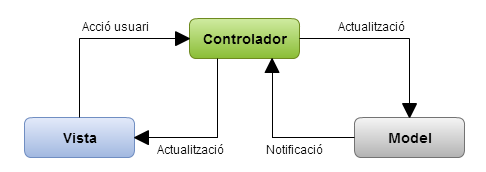
\includegraphics[scale=1]{Memoria/Arquitectura/iOS/patro_mvc.png}
    \caption{Flux de control del patró MVC.}
    \label{fig:patro_mvc}
\end{figure}


El Model representa la informació amb la que el sistema treballa. Les Vistes presenten el model amb el que interactua l'usuari, també conegut com a interfície. El Controladors gestionen els esdeveniments que es capten a les vistes, normalment generats per accions que l'usuari realitza i que impliquen canvis en el model i a la mateixa interfície.


A la figura \ref{fig:patro_mvc} podem veure el flux de control del patró Model Vista Controlador.
\begin{compactitem}
    \item L'usuari realitza una acció en una vista.
    \item El controlador tracta l'acció d'entrada, que pot implicar un canvi en l'estat del model.
    \item El controlador si ho necessita genera una nova vista i s'espera a una altre nova acció de l'usuari.
\end{compactitem}

El patró MVC és un patró que marca tres rols diferenciats i la comunicació que hi ha d'haver entre ells.